\documentclass[a4paper,11pt]{report}

\usepackage{fullpage}

\usepackage{amsmath}
\usepackage{bussproofs}
\usepackage{mathpartir}
\usepackage{prooftrees}
\usepackage{color}
\usepackage{hyperref}
\usepackage{placeins}


% for finite state automata
\usepackage{tikz}
\usetikzlibrary{automata,positioning}

%%%%%%%%%%%%%%%%%%%%%%%%%%%%%%%%%%%%%%%%%%%%%%%%%%%%%%%%%
% Minted
%%%%%%%%%%%%%%%%%%%%%%%%%%%%%%%%%%%%%%%%%%%%%%%%%%%%%%%%%

\usepackage[cache=false]{minted}

%%%%%%%%%% C
\newmintinline{c}{
  fontsize=\small,
  breaklines=true
}

\newminted{c}{
  frame=single,
  framesep=2mm,
  fontsize=\scriptsize,
  mathescape
}

\newminted[ccodeline]{c}{
  frame=single,
  framesep=2mm,
  fontsize=\scriptsize,
  mathescape,
  linenos
}


%%%%%%%%% CMAKE
\newminted{cmake}{
  frame=single,
  framesep=2mm,
  fontsize=\scriptsize,
  mathescape,
  linenos,
  breaklines=true
}

% End minted
%%%%%%%%%%%%%%%%%%%%%%%%%%%%%%%%%%%%%%%%%%%%%%%%%%%%%%%%%


\author{Sylvain Julmy}
\date{\today}

\setlength{\parindent}{0pt}

\begin{document}

\begin{center}
  \Large{
    Operating Systems\\
    Spring 2018
  }
  
  \noindent\makebox[\linewidth]{\rule{\linewidth}{0.4pt}}
  S03
  \noindent\makebox[\linewidth]{\rule{\linewidth}{0.4pt}}

  \begin{flushleft}
    Professor : Philippe Cudré-Mauroux

    Assistant : Ines Arous
  \end{flushleft}
  
  \noindent\makebox[\linewidth]{\rule{\linewidth}{0.4pt}}

  Submitted by Sylvain Julmy
  
  \noindent\makebox[\linewidth]{\rule{\textwidth}{1pt}}
\end{center}

\section*{Exercice 2}

\subsection*{\texttt{Root Disk}}
We use the following command :

\begin{verbatim}
lsblk
\end{verbatim}

In order to obtain the full information about the block devices we have.
Figure~\ref{fig:root} shows the output of the command.

\begin{figure}[ht]
  \centering
  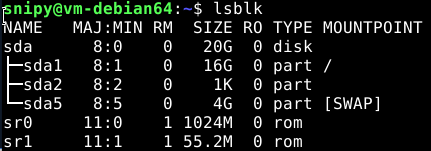
\includegraphics[width=0.6\textwidth]{figures/root_disk}
  \caption{\label{fig:root} Output of the \texttt{lsblk} command.}
\end{figure}

\subsection*{\texttt{Processor Architecture}}
We use the following command :

\begin{verbatim}
lscpu
\end{verbatim}

Figure~\ref{fig:cpu} shows the output of the command.

\begin{figure}[ht]
  \centering
  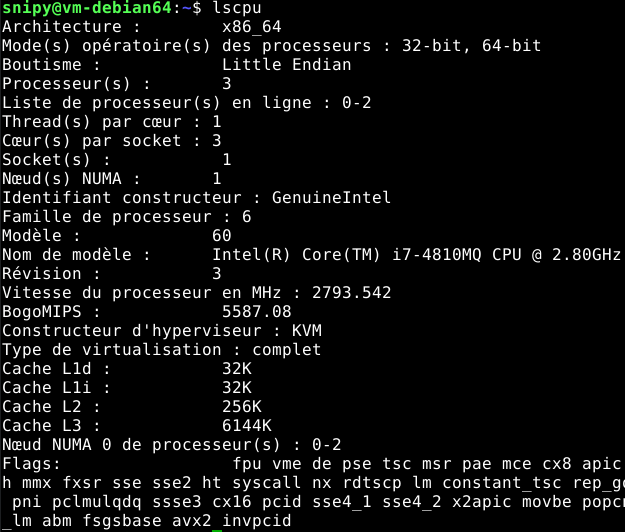
\includegraphics[width=0.6\textwidth]{figures/cpu}
  \caption{\label{fig:cpu} Output of the \texttt{lscpu} command.}
\end{figure}

\subsection*{\texttt{Graphic Card}}
We use the following command :

\begin{verbatim}
lspci -vnn | grep VGA -A 12
\end{verbatim}

\begin{figure}[ht]
  \centering
  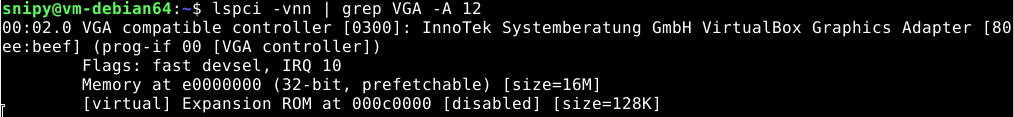
\includegraphics[width=0.9\textwidth]{figures/gc}
  \caption{\label{fig:gc} Output of the \texttt{lspci -vnn | grep VGA -A 12} command.}
\end{figure}

Note : because we are inside a virtual machine, the operating system has no
access to the material directly. So figures~\ref{fig:gc-nat}

\begin{figure}[ht]
  \centering
  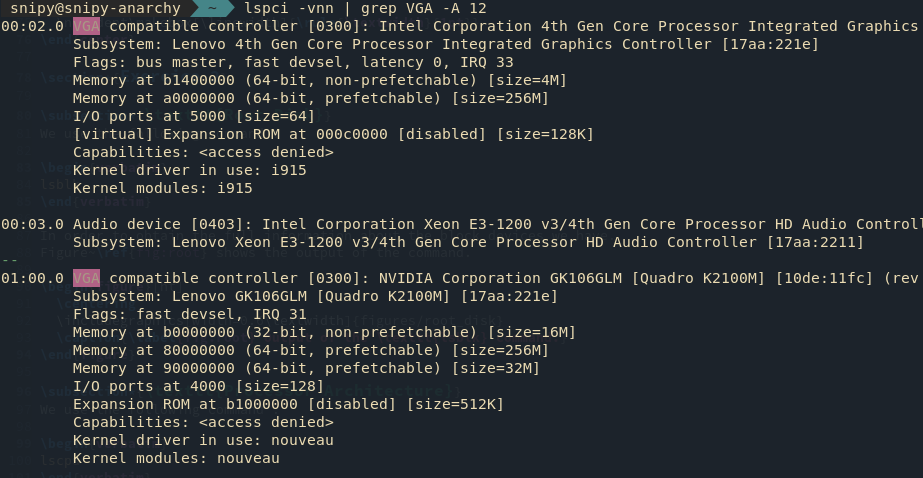
\includegraphics[width=0.9\textwidth]{figures/gc_nat}
  \caption{\label{fig:gc-nat} Output of the \texttt{lspci -vnn | grep VGA -A 12}
    command inside a native installation of linux.}
\end{figure}

\subsection*{\texttt{Memory Size}}
We just look at the file \verb+/proc/meminfo+ to obtain the information.
Figures~\ref{fig:mem} shows the output of the \verb+cat+ command.

\begin{figure}[ht]
  \centering
  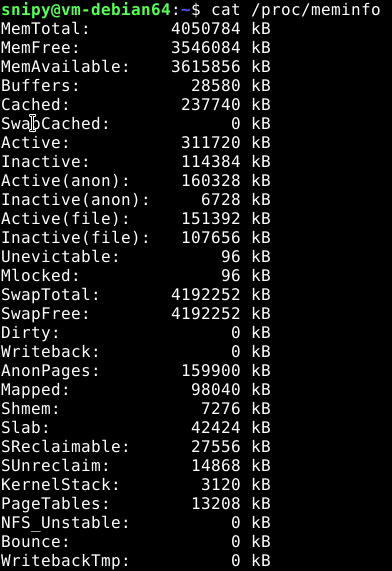
\includegraphics[width=0.6\textwidth]{figures/mem}
  \caption{\label{fig:mem} Output of the \texttt{/proc/meminfo} file.}
\end{figure}

\subsection*{\texttt{Kernel Version}}

We use the following command :

\begin{verbatim}
uname -a
\end{verbatim}

Figure~\ref{fig:mem} shows the output of the \verb+uname -a+ command.

\begin{figure}[ht]
  \centering
  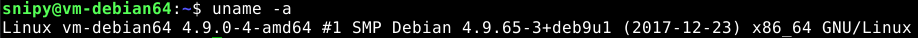
\includegraphics[width=0.6\textwidth]{figures/kernel}
  \caption{\label{fig:mem} Output of the \texttt{uname -a} command.}
\end{figure}

\subsection*{\texttt{Network Card Speed}}

We use the following command (in superuser mode):

\begin{verbatim}
lshw -class network
\end{verbatim}

Figure~\ref{fig:mem} shows the output of the \verb+lshw -class network+ command.

\begin{figure}[ht]
  \centering
  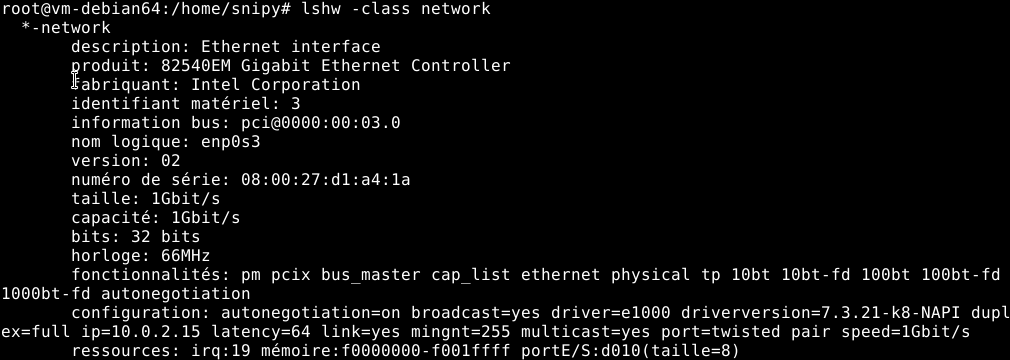
\includegraphics[width=0.9\textwidth]{figures/network}
  \caption{\label{fig:mem} Output of the \texttt{lshw -class network} command.}
\end{figure}

\FloatBarrier

\section*{Exercice 3}

\begin{figure}[ht]
  \centering
  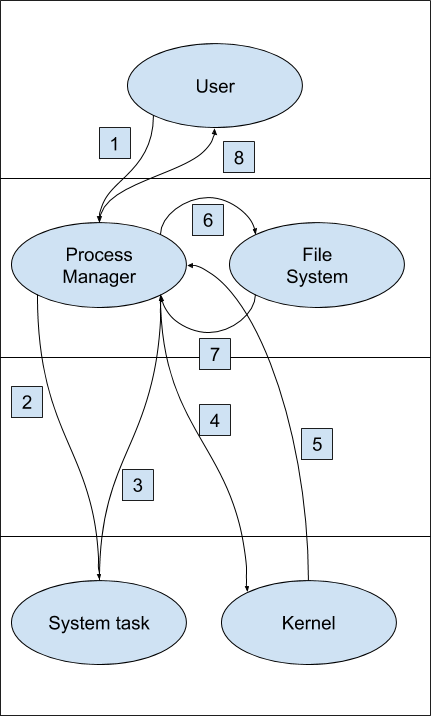
\includegraphics[width=0.6\textwidth]{figures/OS-s03-ex4}
  \caption{\label{fig:fork-path} Path execution of the \texttt{fork()} system
    call in Minix.}
\end{figure}

\FloatBarrier

\newpage

\section*{Exercice 4}

The following C program create two process and each of them are printing their
process id and priority value.

\begin{ccode}
#include <stdio.h>
#include <unistd.h>
#include <sys/resource.h>

void main(void)
{
    int pid;

    pid = fork();
    // from here there are two process

    printf("PID : %d PRIO : %d\n", pid, getpriority(PRIO_PROCESS, 0));
}
\end{ccode}

We use the following CMAKE file in order to compile our program.

\begin{cmakecode}
cmake_minimum_required(VERSION 3.9)
project(OS-S03)

set(CMAKE_C_STANDARD 11)

add_executable(how_nice how_nice.c)
\end{cmakecode}

And one of the output of the program :

\begin{verbatim}
./how_nice
PID : 26835 PRIO : 0
PID : 0 PRIO : 0
\end{verbatim}

\end{document}
